%%%%%%%%%%%%%%%%%%%%%%%%%%%%%%%%%%%%%%%%%
% Document Author: Plinio H. Vargas
% Course: CS-532, Spring 2016 at Old Dominion University
%
% Structured General Purpose Assignment
% LaTeX Template
%
% This template has been downloaded from:
% http://www.latextemplates.com
%
% Original template author:
% Ted Pavlic (http://www.tedpavlic.com)
%
% Note:
% The \lipsum[#] commands throughout this template generate dummy text
% to fill the template out. These commands should all be removed when 
% writing assignment content.
%
%%%%%%%%%%%%%%%%%%%%%%%%%%%%%%%%%%%%%%%%%
%----------------------------------------------------------------------------------------
%	PACKAGES AND OTHER DOCUMENT CONFIGURATIONS
%----------------------------------------------------------------------------------------

\documentclass{article}

\usepackage{fancyhdr} % Required for custom headers
\usepackage{lastpage} % Required to determine the last page for the footer
\usepackage{extramarks} % Required for headers and footers
\usepackage{listings}
\usepackage{graphicx} % Required to insert images
\usepackage{lipsum} % Used for inserting dummy 'Lorem ipsum' text into the template
\usepackage[bookmarks,bookmarksopen,bookmarksdepth=2]{hyperref} % for bookmarks
\usepackage{enumerate}
\usepackage{csquotes} % for quoting things
\usepackage{multirow}
\usepackage{amsmath}
\usepackage{caption}
\usepackage{navigator}%\usepackage{caption}
\usepackage[shortlabels]{enumitem}
\usepackage{lmodern}
\usepackage[utf8]{inputenc}
%\usepackage[table]{xcolor}% http://ctan.org/pkg/xcolo
\usepackage[dvipsnames]{xcolor}
\usepackage{longtable}
\usepackage{textcomp}
\usepackage{url}
\usepackage{import}
\usepackage{float}
\usepackage{dashrule} % for dashline
\usepackage{keystroke}

\lstdefinestyle{numbers}
{ frame=tb,
  language=python,
  aboveskip=3mm,
  belowskip=3mm,
  showstringspaces=false,
  columns=flexible,
  basicstyle={\small\ttfamily},
  numbers=left,
  numberstyle=\tiny\color{gray},
  keywordstyle=\color{blue},
  commentstyle=\color{OliveGreen},
  stringstyle=\color{purple},
  breaklines=true,
  breakatwhitespace=true,
  tabsize=3
}

\lstdefinestyle{nonumbers}
{ frame=shadowbox,
  language=python,
  aboveskip=3mm,
  belowskip=3mm,
  showstringspaces=false,
  columns=flexible,
  basicstyle={\small\ttfamily},
  numbers=none,
  numberstyle=\tiny\color{gray},
  keywordstyle=\color{blue},
  commentstyle=\color{OliveGreen},
  stringstyle=\color{purple},
  breaklines=true,
  breakatwhitespace=true,
  tabsize=3
}

\lstdefinestyle{mybox}
{
	basicstyle={\small\ttfamily},
    numbers=left,
    numberstyle=\tiny\color{gray},
    stepnumber=1,
    numbersep=5pt,
    showspaces=false, % don't show spaces by adding underscores
    showstringspaces=false, % don't underline spaces in strings
    showtabs=false, % don't show tabs with underscores
    frame=shadowbox,
    tabsize=4,
    captionpos=b,
    breaklines=true,
    breakatwhitespace=false,
  	keywordstyle=\color{blue},
	commentstyle=\color{OliveGreen},
  	stringstyle=\color{purple},    
    rulesepcolor=\color{red!20!green!20!blue!20},
    numberbychapter=false,
    stringstyle=\color{purple},
}
% Margins
\topmargin=-0.45in
\evensidemargin=0in
\oddsidemargin=0in
\textwidth=6.5in
\textheight=9.0in
\headsep=0.25in 

\linespread{1.1} % Line spacing
\newcommand*{\medtau}{\mathbin{\scalebox{1.5}{$\tau$}}}% increase size of tau
\newcommand*{\medtaub}{\mathbin{\scalebox{1.5}{$\tau_b$}}}% increase size of tau_b
\newcommand\multibrace[3]{\rdelim\}{#1}{3mm}[\pbox{#2}{#3}]}

% Set up the header and footer
\pagestyle{fancy}
\lhead{\hmwkAuthorName} % Top left header
\chead{\hmwkShortClass\ (\hmwkClassInstructor\ \hmwkClassTime): \hmwkShortTitle} % Top center header
%\rhead{\firstxmark} % Top right header
\rhead{} % Top right header
\lfoot{\lastxmark} % Bottom left footer
\cfoot{} % Bottom center footer
\rfoot{Page\ \thepage\ of\ \pageref{LastPage}} % Bottom right footer
\renewcommand\headrulewidth{0.4pt} % Size of the header rule
\renewcommand\footrulewidth{0.4pt} % Size of the footer rule

\setlength\parindent{0pt} % Removes all indentation from paragraphs

%----------------------------------------------------------------------------------------
%	DOCUMENT STRUCTURE COMMANDS
%	Skip this unless you know what you're doing
%----------------------------------------------------------------------------------------

% Header and footer for when a page split occurs within a problem environment
\newcommand{\enterProblemHeader}[1]{
\nobreak\extramarks{#1}{#1 continued on next page\ldots}\nobreak
\nobreak\extramarks{#1 (continued)}{#1 continued on next page\ldots}\nobreak
}

% Header and footer for when a page split occurs between problem environments
\newcommand{\exitProblemHeader}[1]{
\nobreak\extramarks{#1 (continued)}{#1 continued on next page\ldots}\nobreak
\nobreak\extramarks{#1}{}\nobreak
}

\setcounter{secnumdepth}{0} % Removes default section numbers
\newcounter{homeworkProblemCounter} % Creates a counter to keep track of the number of problems

\newcommand{\homeworkProblemName}{}
\newenvironment{homeworkProblem}[1][Problem \arabic{homeworkProblemCounter}]{ % Makes a new environment called homeworkProblem which takes 1 argument (custom name) but the default is "Problem #"
\stepcounter{homeworkProblemCounter} % Increase counter for number of problems
\renewcommand{\homeworkProblemName}{#1} % Assign \homeworkProblemName the name of the problem
\section{\homeworkProblemName} % Make a section in the document with the custom problem count
\enterProblemHeader{\homeworkProblemName} % Header and footer within the environment
}{
\exitProblemHeader{\homeworkProblemName} % Header and footer after the environment
}

\newcommand{\problemAnswer}[1]{ % Defines the problem answer command with the content as the only argument
\noindent\framebox[\columnwidth][c]{\begin{minipage}{0.98\columnwidth}#1\end{minipage}} % Makes the box around the problem answer and puts the content inside
}

\newcommand{\homeworkSectionName}{}
\newenvironment{homeworkSection}[1]{ % New environment for sections within homework problems, takes 1 argument - the name of the section
\renewcommand{\homeworkSectionName}{#1} % Assign \homeworkSectionName to the name of the section from the environment argument
\subsection{\homeworkSectionName} % Make a subsection with the custom name of the subsection
\enterProblemHeader{\homeworkProblemName\ [\homeworkSectionName]} % Header and footer within the environment
}{
\enterProblemHeader{\homeworkProblemName} % Header and footer after the environment
}
   
%----------------------------------------------------------------------------------------
%	NAME AND CLASS SECTION
%----------------------------------------------------------------------------------------

\newcommand{\hmwkTitle}{\\Assignment\ \#5: \\The \enquote{Karate Club (Zachary, 1977)}} % Assignment title
\newcommand{\hmwkShortTitle}{Assignment 5} % Assignment title
\newcommand{\hmwkDueDate}{Thursday,\ March 3,\ 2016} % Due date
\newcommand{\hmwkClass}{CS-432/532 Introduction to Web Science} % Course/class
\newcommand{\hmwkShortClass}{CS-432/532 Web Science} % Course/class
\newcommand{\hmwkClassTime}{- Spring 2016} % Class/lecture time
\newcommand{\hmwkClassInstructor}{Dr.  Michael L. Nelson} % Teacher/lecturer
\newcommand{\hmwkAuthorName}{Plinio Vargas} % Your name
\newcommand{\hmwkAuthorEmail}{pvargas@cs.odu.edu} % Your name
%------------------------------------------------------------
% Algorithm declaration
%------------------------------------------------------------
\lstnewenvironment{algorithm}[1][] %defines the algorithm listing environment
{   
    %\refstepcounter{nalg} %increments algorithm number
    \captionsetup{labelsep=colon} %defines the caption setup for: it ises label format as the declared caption label above and makes label and caption text to be separated by a ':'
    \lstset{ %this is the stype
        frame=tB,
        numbers=left, 
        mathescape=true,
        numberstyle=\tiny,
        basicstyle={\small\ttfamily}, 
        keywordstyle=\color{blue}\bfseries\em,
        keywords={,input, output, return, 
                   datatype, function, in, 
                   if, else, for, foreach, 
                   while, write, begin, end, 
        } %add the keywords you want, or load a language as Rubens explains in his comment above.
        numbers=left,
        xleftmargin=.04\textwidth,
        #1 % this is to add specific settings to an usage of this environment (for instnce, the caption and referable label)
    }
}
{}
%----------------------------------------------------------------------------------------
%	TITLE PAGE
%----------------------------------------------------------------------------------------

\title{
\vspace{2in}
\textmd{\textbf{\hmwkClass:\ \hmwkTitle}}\\
\normalsize\vspace{0.1in}\small{Due\ on\ \hmwkDueDate}\\
\vspace{0.1in}\large{\textit{\hmwkClassInstructor\ }}
\vspace{3in}
}

\author{\textbf{\hmwkAuthorName} \\ \hmwkAuthorEmail}
\date{} % Insert date here if you want it to appear below your name

%----------------------------------------------------------------------------------------
%	EMBEDDED FILE
%----------------------------------------------------------------------------------------
\embeddedfile{KarateClub}{../KarateClub.py}
\embeddedfile{DrawOriginalClub}{../DrawOriginalClub.py}
%----------------------------------------------------------------------------------------
%	START OF DOCUMENT
%----------------------------------------------------------------------------------------
\begin{document}

\clearpage\maketitle
\thispagestyle{empty}

%----------------------------------------------------------------------------------------
%	TABLE OF CONTENTS
%----------------------------------------------------------------------------------------

%\setcounter{tocdepth}{1} % Uncomment this line if you don't want subsections listed in the ToC

\newpage
\clearpage\tableofcontents
\listoffigures
\lstlistoflistings
\listoftables

\thispagestyle{empty}
\newpage
\setcounter{page}{1}

%----------------------------------------------------------------------------------------
%	Problem 1
%----------------------------------------------------------------------------------------
\begin{homeworkProblem} % Custom section title
\vspace*{10pt} % Question
We know the result of the Karate Club (Zachary, 1977) split.
Prove or disprove that the result of split could have been predicted by the weighted graph of social interactions.  How well does the mathematical model represent reality?\\

Generously document your answer with all supporting equations, code, graphs, arguments, etc.

\subsection{1.1 Approach}
Social interaction among individuals can be represented as a graph, where nodes signify a particular individual of the social network, and edges between nodes represent some type of relationship between them. An individual may enter the social network influenced by a node belonging to the network or by other means. If the inclusion into the network was influenced by a node within the network, the bond between those two nodes is much stronger than if they just associated by mere interaction in the network.\\

Similarly, disputes and differences may cause rupture in a relationship, this could be represented as removing an edge between two nodes in the graph. This conflict may be so common  among other members within a social network that a collection of edges removal could translate in splitting a group (network) into two or more separate entities. In $graph$ studies, particularly undirected $graphs$ (which is our case), if a node can reach other nodes within the $graph$, it is denoted as a $connected\ component$. We are going to use this definition to check if at any point after removing an edge the $graph$, fulfills the characteristic of a $connected\ component$.\\

Then, if the number of connected components in an original graph $G$ is equal to one (1), we will be able to check if $G$ has split after the removal of an edge ($u, v$) between nodes $u$ and $v$ that are part of $G$ by testing the condition:
\begin{equation}\label{eq:component}
	\forall n\ \in G\ where\ n\ is\ a\ node\ of\ G.\ n\ can\ traverse\ \to |G| - 1\ nodes
\end{equation}

We are going to be emulating the breaking of the well known and studied \enquote{Karate Club}\cite{kclub}. An important concept identified in the original study\cite{kclub} is how the information flowed within the network. As friction began to arise meeting were called by a faction within the club, which was not interested that rival faction received the information. However, since the network is still in one $connected-component$, all the members were able somehow get the information. The leader of a faction who usually passed the information was labeled as the $source$, and the leader of a rival faction was labeled as $sink$.\\

In a single split of $G=(V, E)$ we will create an identical graph $G'=(V', E')$ where:
\begin{equation}\label{eq:sink}
	sink = max(|v_1|, |v_2|, \cdots, |v_n|)
\end{equation}
Where $v$ is a vertex in $G'$ and $n$ is the number of vertices in the graph. To find the source, we make $G' = G' - sink - all\ edges (u', v')\ adjecent\ to\ sink$. Then $source$ is:

	$$n = G.size$$
\begin{equation}\label{eq:source}
	source = max(|v_1|, |v_2|, \cdots, |v_n|)
\end{equation}
Where $v$ is a vertex in $G'$, and $n$ is the number of vertices in the new graph.\\

Equations \eqref{eq:sink} and \eqref{eq:source} are relevant in determining edges removal. Since splitting the network consists of making invalid the condition of equation \eqref{eq:component}, we are trying to break the edges not strongly related to $source$ that are an information flow bridge to $sink$.

Although the solution on how the Karate Club \cite{kclub} splits into two different groups has been very well documented, and many resources are available to simulate and predict the outcome, we need to \enquote{Remember that all models are wrong; the practical question is how wrong do they have to be to not be useful}\cite{box} and \enquote{Essentially, all models are wrong, but some are useful}\cite{box}. Also the compared simulation model was not able to have 100\% accuracy. Node \#9 was expected to split to be color coded white, but other factors not input in the graphs weighted more than the expected result.\\

Borrowing from week 6's ODU Spring-16 Web Science class slide number 66, it is easy to visualize actual result. If we were to separate the network below into two different ones, we would need to cut the edges joining two nodes with different color.

\begin{figure}[!h]
\center
\caption{Karate Club Split-Color-Coded Nodes} \label{fig:1}
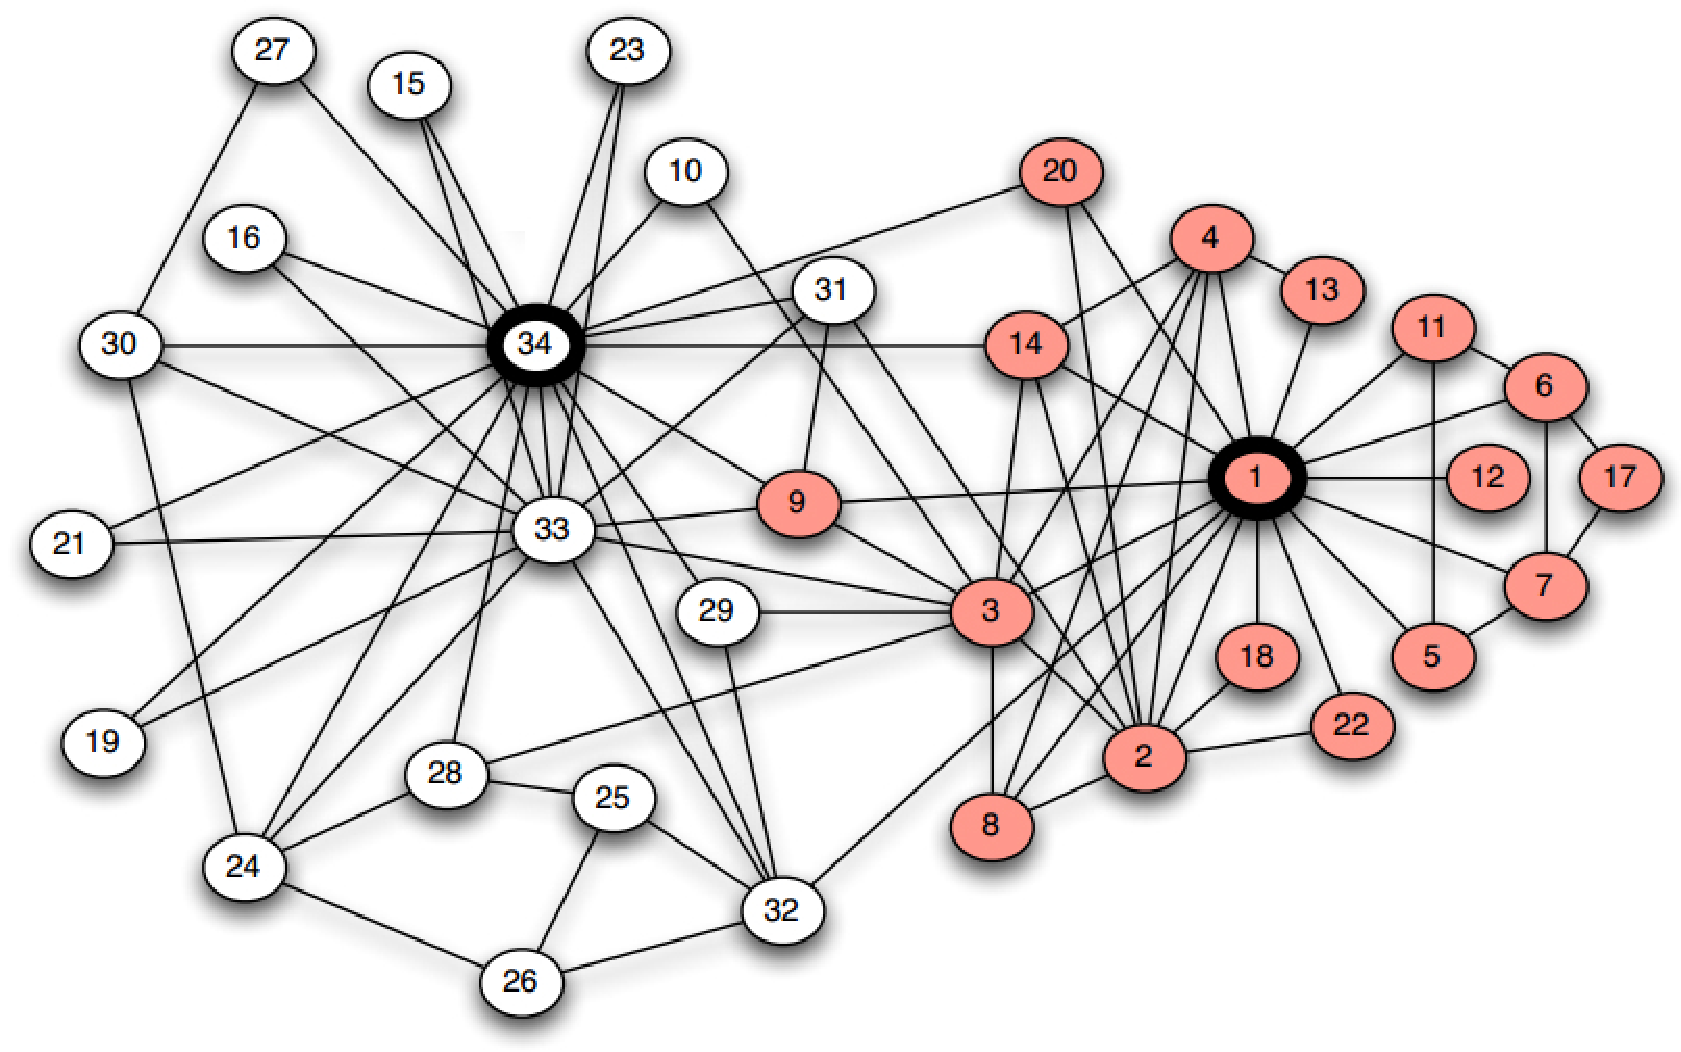
\includegraphics[scale=.5]{images/slide-66.pdf}
\caption*{\scriptsize Figure \ref{fig:1} shows social interactions among members of the club outside the facility. The color coded nodes represent how the grouping of nodes after the club split.}
\end{figure}

\newpage
Making the split when we don't have color code node is not as simple. 
\\
\begin{figure}[!h]
\center
\caption{Karate Club Homogeneous Color Nodes} \label{fig:2}
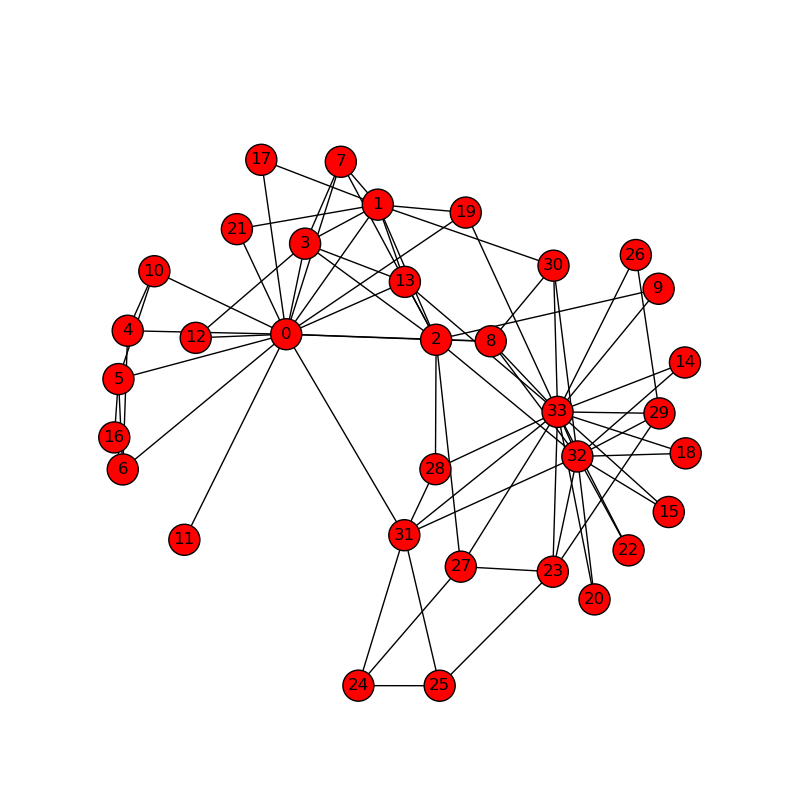
\includegraphics[scale=.5]{images/original-club.png}
\caption*{\scriptsize Figure \ref{fig:2} shows social interactions among members of the club outside the facility. Although this graph is not that complex, it is not trivial to figure out where the faction split after node colors become homogeneous. The graph was generated using $matplotlib$ Python library. The code for graphic generation is included in $<DrawOriginalClub.py>$ which is attached to this document.}
\end{figure}

The Python library \textbf{\textit{networkx}} was very useful to a create our model. Many graph's functionality, such as creating a node, adding adjacent vertices, or removing edges is easy to handle with this library. Although the data for \cite{kclub} is available in \textbf{\textit{networkx}}. The data to create the graph was upload as a matrix from \cite{club-data} with the purpose of manipulating $source-sink$ rows in the graph.

\newpage
\subsection{1.2 Solution}
The Python application $<KarateClub.py>$ attached to this document was implemented to create our social network splitting model. 

\lstinputlisting[language=Python,
                 style=mybox, 
                 captionpos=t,
                 caption={Finding Source-Sink in Graph},
                 label=listing:Grep,
				 linerange={72-78},
				 firstnumber=72                 
                 ]
{../KarateClub.py}

\vspace{5mm}
To find $sink$ and $source$ we can apply equations \eqref{eq:sink} and \eqref{eq:source} respectively. First, line 73 gets all vertices in our graph $G$. We get the vertex with highest degree for $sink$. Finally, we delete vertex containing the sink value (line 77). The next vertex with highest degree becomes our $source$.\\

\begin{figure}[!h]
\center
\caption{Karate Club Showing Sink-Source Nodes} \label{fig:3}
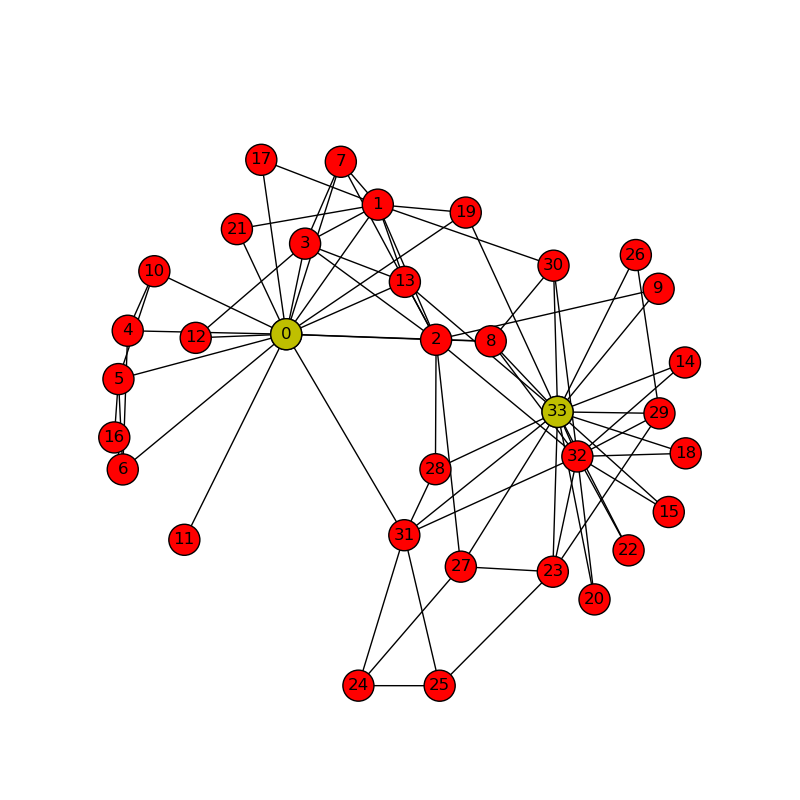
\includegraphics[scale=.5]{images/original-sink-soruce.png}
\caption*{\scriptsize Figure \ref{fig:3} shows social interactions among members of the club outside the facility. It is still not trivial to figure out where the faction will split. The graph provides a much richer view than Figure \ref{fig:2}. We can have a general ideal of the outcome by focusing on the nodes color-coded  yellow for $source$ (0) and $sink$ (33). The graph was generated using $matplotlib$ Python library. The code for graphic generation is included in $<DrawOriginalClub.py>$ which is attached to this document.}
\end{figure}

A python implementation Girvan-Newman Algorithm was extracted from \cite{gn-algorithm}. Minor modifications were made to adapt our python3 environment. The heart of our solution resides in the listing below:

\lstinputlisting[language=Python,
                 style=mybox, 
                 captionpos=t,
                 caption={Calculating Edge Betweenness for Graph $G$},
                 label=listing:Grep,
				 linerange={80-95},
				 firstnumber=80                 
                 ]
{../KarateClub.py}

\vspace*{5mm}
Line 80 initializes the number of components in $G$ which originally is one (1). Lines 85-95 is a while-loop that verifies if equation \eqref{eq:component} is satisfied. The number of connected components in $G$ is modified after the edge with the highest flow has been found (line 92). Lines 91-94 iterates through edges in $G$ and removes edges ($u, v$) which has the highest betweeness value. The time complexity for this algorithm is $O(|V| |E|)$.\\

Running $<KarateClub.py>$ shows that 11 iterations to remove edges in $G$ were required to have 2 connected-components in the graph. The specific edges removed from $G$ are shown below:\\

\begin{lstlisting}[style=nonumbers]
Starting Time: Wed,  Mar 02, 2016 at 19:39:14
(0, 31)
(0, 2)
(0, 8)
(13, 33)
(19, 33)
(2, 32)
(1, 30)
(1, 2)
(2, 3)
(2, 13)
(2, 7)

End Time:  Wed,  Mar 02, 2016 at 19:39:14
Execution Time: 0.26 seconds
\end{lstlisting}

Drawing the Graph after creating more than one connected component is represented below:

\newpage
\begin{figure}[!h]
\center
\caption{Karate Club Split Graph Projection} \label{fig:4}
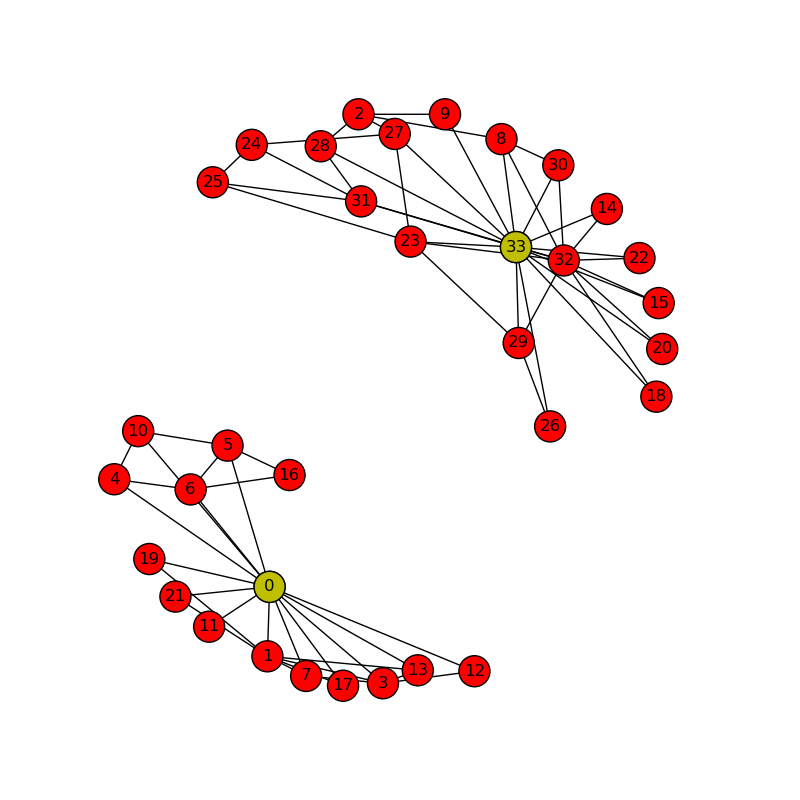
\includegraphics[scale=.5]{images/club-2splits.png}
\caption*{\scriptsize Figure \ref{fig:4} shows the projected Karate Club separation. Since we already know the results from Figure \ref{fig:1},  to calculate how accurate our projection is, we can count the number of accurate vertices for both groups and divide that number into the total number of vertices in the graph.}
\end{figure}

Node comparison has to be defined since Figure \ref{fig:1} starts with node 1, while we start with node 0. Thus, when comparing with Figure \ref{fig:1}, we will be adding 1 to the compared node, but the listing of node discrepancy will be based on nodes from Figure \ref{fig:4}.\\

\subsection{1.3 Comparing Results}
Comparing Figure \ref{fig:1} and Figure \ref{fig:4} yields interesting results. The $source$ faction properly projected the following nodes:\\

\{0,1,3,4,5,6,7,10,11,12,13,16,18,19,21\}\\

Only two (2) nodes were mis-projected resulting in  a confidence level of 32/34 or 94\%. Using weighted adjacent matrix data in Table \ref{tab:table2} with the same algorithm, yielded the same result.

\end{homeworkProblem}

%----------------------------------------------------------------------------------------
%	Problem 2 Extra Credit 1 Point
%----------------------------------------------------------------------------------------
\newpage
\begin{homeworkProblem}[Problem 2 - Extra Credit]
We know the group split in two different groups.  Suppose the disagreements in the group were more nuanced \texttt{--} what would the clubs look like if they split into groups of 3, 4, and 5?
\subsection{2.1 Approach}
We are going to use the same approach as in 1.1, however in line 85 we will increase the number of connected components by one, depending on the desire output. For example, if we desire 3 connected component result, we may modify line 85 as follows:

\begin{lstlisting}[style=mybox, firstnumber=85, language=python]
while ncomp <= init_ncomp + 1:
\end{lstlisting}

\subsection{2.2 Karate Club 3-Split Solution}
The following edges were removed to obtain 3 separate connected components from the original graph:

\begin{lstlisting}[style=nonumbers]
Starting Time: Thu,  Mar 03, 2016 at 19:35:20
(0, 31)
(0, 2)
(0, 8)
(13, 33)
(19, 33)
(2, 32)
(1, 30)
(1, 2)
(2, 3)
(2, 13)
(2, 7)
(9, 33)
(27, 33)
(2, 9)

End Time:  Thu,  Mar 03, 2016 at 19:35:21
Execution Time: 0.29 seconds
\end{lstlisting}

\newpage
\begin{figure}[!h]
\center
\caption{Karate Club 3-Split Graph Projection} \label{fig:5}
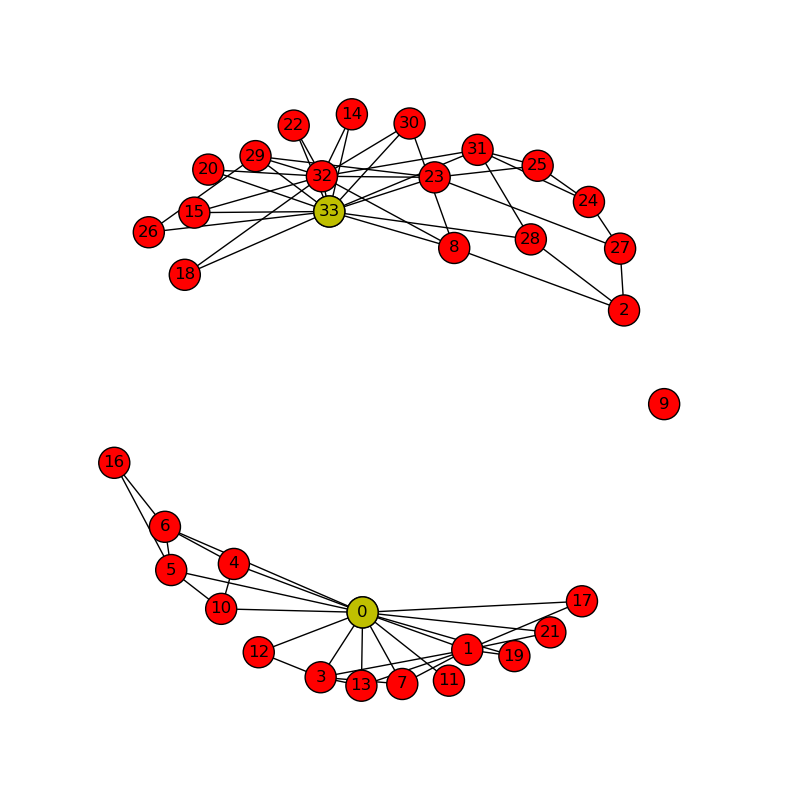
\includegraphics[scale=.5]{images/club-3splits.png}
\caption*{\scriptsize Figure \ref{fig:5} shows the projected Karate Club separation in three (3) different groups. Only vertex 9 was separated from the first split, and it took three extra edges removal to make node 9 and independent component.}
\end{figure}

\subsection{2.3 Karate Club 4-Split Solution}
The following edges were removed to obtain 4 separate connected components from the original graph:

\begin{lstlisting}[style=nonumbers]
Starting Time: Thu,  Mar 03, 2016 at 19:40:20
(0, 31)
(0, 2)
(0, 8)
(13, 33)
(19, 33)
(2, 32)
(1, 30)
(1, 2)
(2, 3)
(2, 13)
(2, 7)
(9, 33)
(27, 33)
(2, 9)
(0, 6)
(0, 5)
(0, 4)
(0, 10)

End Time:  Thu,  Mar 03, 2016 at 19:40:20
Execution Time: 0.32 secondss
\end{lstlisting}

\begin{figure}[!h]
\center
\caption{Karate Club 4-Split Graph Projection} \label{fig:6}
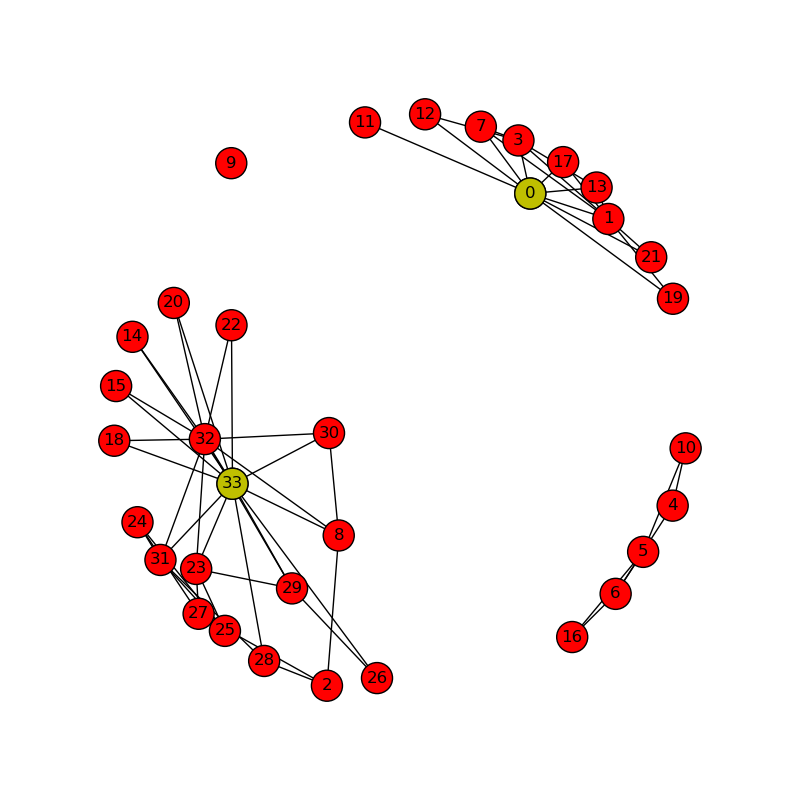
\includegraphics[scale=.5]{images/club-4splits.png}
\caption*{\scriptsize Figure \ref{fig:6} shows the projected Karate Club separation in four (4) different groups. Overall, 18 edges were removed to create a four-way split.}
\end{figure}

\subsection{2.4 Karate Club 5-Split Solution}
The following edges were removed to obtain 5 separate connected components from the original graph:

\begin{lstlisting}[style=nonumbers]
Starting Time: Thu,  Mar 03, 2016 at 19:42:30
(0, 31)
(0, 2)
(0, 8)
(13, 33)
(19, 33)
(2, 32)
(1, 30)
(1, 2)
(2, 3)
(2, 13)
(2, 7)
(9, 33)
(27, 33)
(2, 9)
(0, 6)
(0, 5)
(0, 4)
(0, 10)
(31, 33)
(31, 32)
(28, 33)
(23, 25)
(23, 27)
(2, 8)

End Time:  Thu,  Mar 03, 2016 at 19:42:31
Execution Time: 0.37 seconds
\end{lstlisting}

\begin{figure}[!h]
\center
\caption{Karate Club 5-Split Graph Projection} \label{fig:7}
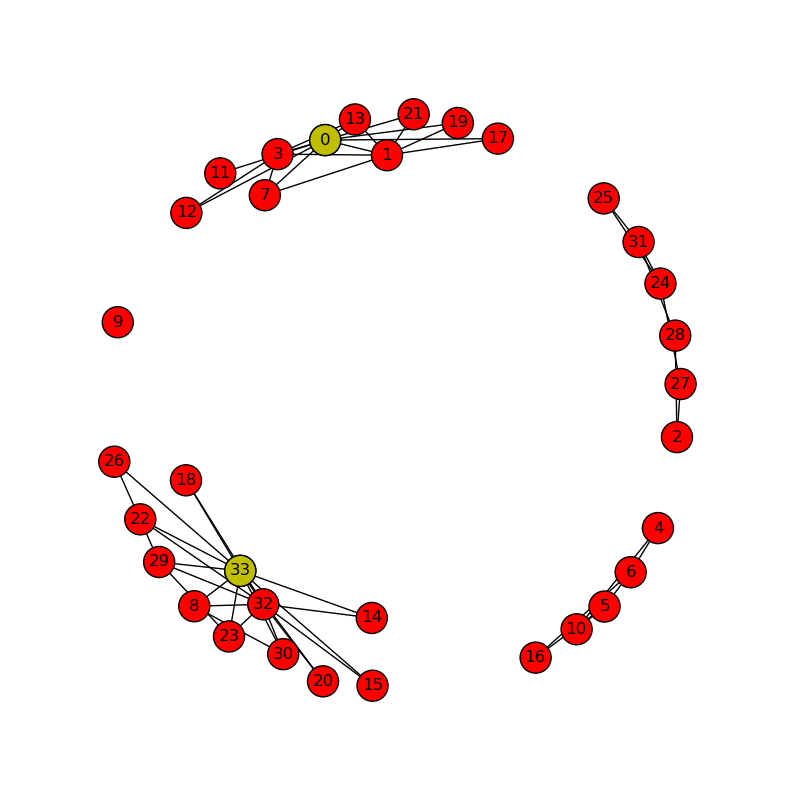
\includegraphics[scale=.5]{images/club-5splits.png}
\caption*{\scriptsize Figure \ref{fig:7} shows the projected Karate Club separation in five (5) different groups. Overall, 24 edges were removed to create a five-way split.}
\end{figure}


\end{homeworkProblem}

%----------------------------------------------------------------------------------------
%	Tables
%----------------------------------------------------------------------------------------
\import{./}{tables.tex}
%----------------------------------------------------------------------------------------
%	Bibliography
%----------------------------------------------------------------------------------------
\newpage
\begin{thebibliography}{9}
%\bibitem{Lutz} 
%Lutz, Mark (2013). List and Dictionaries. \textit{Learning Python} (5th ed.). (pp. %262-263). Sebastopol, CA: O'Reilly Media.
%
\bibitem{kclub}
Karate Club (Zachary, 1977). (n.d.) Retrieved February 27, 2016, from \url{http://aris.ss.uci.edu/~lin/76.pdft}

\bibitem{box}
Box, G. E. P., and Draper, N. R., (1987), \textit{Empirical Model Building and Response Surfaces}p.74, p.424, John Wiley \& Sons, New York, NY.

\bibitem{club-data}
Karate Club Data Set. (n.d.) Retrieved March 2, 2016, from \url{http://vlado.fmf.uni-lj.si/pub/networks/data/ucinet/zachary.dat/}

\bibitem{gn-algorithm}
Python Girvan-Newman Algorithm. (n.d.) Retrieved March 2, 2016, from \url{https://github.com/kjahan/community/blob/master/cmty.pyl/}
\end{thebibliography}
\end{document}
